\documentclass[12pt,oneside,listof=totoc,paper=a4,headings=small]{scrbook}
% Nützliche Packages für die Gestaltung und allgemeine Konfiguration des Dokuments
% -----------------------------------

% Allgemeine Formatierungen
\usepackage[ngerman]{babel}			% neue deutsche Rechtschreibung
\usepackage[utf8]{inputenc} 		% Umlaute im Text
\usepackage[T1]{fontenc}
\usepackage{xspace}                 % Vermeidung von "ineinanderfallenden f's", wie z.B. bei Schifffahrt
\usepackage{url}		            % korrekte Anzeige/Umbruch von URLs
\usepackage{listings}               % z.B. nützlich zum Einbinden von Quellcode
\usepackage{hyperref} 				% für Hyperlinks in PDF-Dokumenten 
\usepackage{lmodern}
\usepackage{enumerate}
\usepackage{csquotes}
\usepackage{tabularray}
\usepackage{listings}
\usepackage{xcolor}

% Kopfzeile
\usepackage[headsepline,manualmark]{scrlayer-scrpage}
\clearpairofpagestyles
\ohead{\pagemark}
\ihead{\headmark}
\automark{chapter}
\pagestyle{scrheadings}

% Seitenspiegel
\usepackage[left=25mm,right=20mm,top=25mm,bottom=25mm]{geometry}

\definecolor{codegreen}{rgb}{0,0.6,0}
\definecolor{codegray}{rgb}{0.5,0.5,0.5}
\definecolor{codepurple}{rgb}{0.58,0,0.82}
\definecolor{codeorange}{rgb}{1,0.5,0}
\definecolor{backcolour}{rgb}{0.95,0.95,0.92}

\renewcommand{\lstlistingname}{Code-Beispiel}

\lstdefinelanguage{TypeScript}{
	sensitive=true,
	morecomment=[l]{//},
	morecomment=[s]{/*}{*/},
	morestring=[b]",
	keywords=[1]{let, const, break, case, catch, class, const, continue, debugger, default, delete, do, else, enum, export, extends, finally, for, function, if, import, in, instanceof, new, return, super, switch, this, throw, try, typeof, var, void, while, with},
	keywordstyle=[1]\color{blue},
	keywords=[2]{true, false, null,console},
	keywordstyle=[2]\color{codepurple},
	keywords=[3]{string, number, boolean, any, void},
	keywordstyle=[3]\color{codeorange}\bfseries,
	identifierstyle=\color{black},
	commentstyle=\color{gray}\textit,
	stringstyle=\color{codegreen},
	morestring=[b]',
	morestring=[b]`,
}


\lstdefinestyle{mystyle}{
	backgroundcolor=\color{backcolour},   
	commentstyle=\color{codegreen},
	keywordstyle=\color{blue},
	numberstyle=\tiny\color{codegray},
	stringstyle=\color{codepurple},
	basicstyle=\ttfamily\footnotesize,
	breakatwhitespace=false,         
	breaklines=true,                 
	captionpos=b,                    
	keepspaces=true,                 
	numbers=left,                    
	numbersep=5pt,                  
	showspaces=false,                
	showstringspaces=false,
	showtabs=false,                  
	tabsize=2
	}

\lstset{style=mystyle}

% Literatur
\usepackage[backend=biber, %% Hilfsprogramm "biber" (statt "biblatex" oder "bibtex")
            style=numeric, %% Zitierstil (siehe Dokumentation, bitte mit Betreuer absprechen)
            natbib=true, %% Bereitstellen von natbib-kompatiblen Zitierkommandos
            hyperref=true, %% hyperref-Paket verwenden, um Links zu erstellen
]{biblatex}

% Einbindung der Literatur-Datenbank
\addbibresource{./Literatur/quellen.bib}

% Grafiken
\usepackage{graphicx} 				% Grafiken einfügen (pdf,png - aber jpg vermeiden)
\graphicspath{{./Bilder/}}          % Pfad zu den Bildern

% Tabellen
\usepackage{booktabs} 				% bessere Gestaltung von Tabellen
\usepackage{longtable} 				% für bessere Tabellen über mehrere Seiten

% Koma-Script Kompatibilität
\usepackage{scrhack}



% Das Dokument selbst mit seinen Bestandteilen
% --------------------------------------------
\begin{document}
\frontmatter 
    % Titelseite soll keine Kopf oder Fußzeile haben
\thispagestyle{empty}



\vspace*{-20mm}
\begin{flushright}

\includegraphics[width=0.5\textwidth]{Bilder/LogoHS.png}
\end{flushright}


\vspace*{2cm}

% Alle Elemente sollen zentriert sein
\begin{center}
% Art der Arbeit => (Bachelorarbeit , Masterarbeit, Studienarbeit)
{\Large \textbf{Seminar}}\\ 



\vspace{1cm}

% Titel der Arbeit 
{\Large \bfseries Refactoring in der Softwareentwicklung\\ 
	Sommersemester 2024\\
	bei Prof. Dr. Georg Hagel\\}

\vspace*{1cm}

{\large five lines of code (Christian Clausen)\\[1mm]}

\vspace{1.5cm}

% Name des/der Autors/Autoren
{\large Thema: Fogle der Struktur im Code}\\[40mm]

\end{center}

\vfill

% Aufgabensteller, Kontaktdaten und Abgabetermin
\parbox{120mm}{
\begin{tabbing}
Name, Vorname \hspace{2cm} \= Heiserer Valentin\\
Matrikelnummer             \> 453990\\[4mm]
Studiengang                  \> Bachelor Informatik\\
Semester                  \> Sommersemester 2024\\
\end{tabbing}
}

 				    % Titelblatt
%    \newpage
\thispagestyle{empty}

% Bitte hier keine Änderungen vornehmen, sondern vollständig handschriftlich ausfüllen

\noindent  {\Large \textbf{Sperrvermerk}}\\ 

\vspace*{2cm}
\bfseries
\noindent Die nachfolgende Arbeit enthält vertrauliche Informationen und Daten der Firma
VeryBest GmbH. 

\medskip
\noindent Veröffentlichungen oder Vervielfältigungen - auch nur auszugsweise oder in
elektronischer Form - sind ohne ausdrückliche schriftliche Genehmigung der
Firma VeryBest GmbH nicht gestattet.
\medskip

\noindent Die Sperrfrist gilt bis zum 31. Dezember 20XY.

\medskip
\noindent Die Arbeit darf bis zum Ablauf der Sperrfrist nur für Prüfungszwecke verwendet
werden.
\normalfont 			% Sperrvermerk (nur falls von Firma verlangt)
    \newpage

\vspace*{1cm}

\begin{center}
    \textbf{Kurzzusammenfassung}
\end{center}

\vspace*{1cm}

\noindent 
Dieser Blindtext zeigt den ungefähren Umfang des deutschen Abstract.Lorem ipsum dolor sit amet, consectetuer adipiscing elit. Aenean commodo ligula eget dolor. Aenean massa. Cum sociis natoque penatibus et magnis dis parturient montes, nascetur ridiculus mus. Donec quam felis, ultricies nec, pellentesque eu, pretium quis, sem. Nulla consequat massa quis enim. Donec pede justo, fringilla vel, aliquet nec, vulputate eget, arcu. In enim justo, rhoncus ut, imperdiet a, venenatis vitae, justo. Nullam dictum felis eu pede mollis pretium. Integer tincidunt. Cras dapibus. Vivamus elementum semper nisi. Aenean vulputate eleifend tellus. Aenean leo ligula, porttitor eu, consequat vitae, eleifend ac, enim. Aliquam lorem ante, dapibus in, viverra quis, feugiat a, tellus. Phasellus viverra nulla ut metus varius laoreet. Quisque rutrum. Aenean imperdiet. Etiam ultricies nisi vel augue. Curabitur ullamcorper ultricies nisi. Nam eget dui. Etiam rhoncus.  	% Abstract
    \tableofcontents 					            % Inhaltsverzeichnis
    \clearpage
    \listoffigures  					 	        % Abbildungsverzeichnis
    \clearpage
    \listoftables						            % Tabellenverzeichnis 
    \clearpage
% ----------------------------------------------
\mainmatter 						% die einzelnen Kapitel, bei Bedarf weitere *.tex Dateien erzeugen und hier einbinden
    \chapter{Einleitung}

Donec quam felis, ultricies nec, pellentesque eu, pretium quis, sem. Nulla consequat massa quis enim. Donec pede justo, fringilla vel, aliquet nec, vulputate eget, arcu. In enim justo, rhoncus ut, imperdiet a, venenatis vitae, justo. Nullam dictum felis eu pede mollis pretium. Integer tincidunt. Cras dapibus. Vivamus "`elementum semper nisi"' \cite{Fischer.2010b}. Aenean vulputate eleifend tellus. Aenean leo ligula, porttitor eu, consequat vitae, eleifend ac, enim. Aliquam lorem ante, dapibus in, viverra quis, feugiat a, tellus. Phasellus viverra nulla ut metus varius laoreet. Quisque rutrum. Aenean imperdiet. Etiam ultricies nisi vel augue. Curabitur ullamcorper ultricies nisi. 


\section{Forschungsfragen}
Vestibulum fringilla pede sit amet augue. In turpis. Pellentesque posuere. Praesent turpis. Aenean posuere, tortor sed cursus feugiat, nunc augue blandit nunc, eu sollicitudin urna dolor sagittis lacus \cite[S. 33-39]{Brambilla.2012}. Donec elit libero, sodales nec, volutpat a, suscipit non, turpis. Nullam sagittis. Suspendisse pulvinar, augue ac venenatis condimentum, sem libero volutpat nibh, nec pellentesque velit pede quis nunc. Vestibulum ante ipsum primis in faucibus orci luctus et ultrices posuere cubilia Curae; Fusce id purus. Ut varius tincidunt libero. Phasellus dolor.  
\begin{figure}
	\centering
		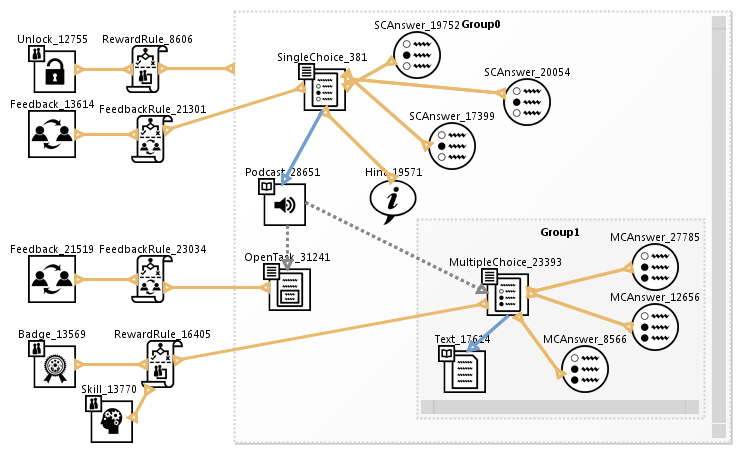
\includegraphics[width=0.7\textwidth]{Bilder/emendo.png}
	\caption{Beispiel 1 zum Einfügen einer Grafik}
	\label{fig:bsp1}
\end{figure}

In ac felis quis tortor malesuada pretium. Pellentesque auctor neque nec urna. Proin sapien ipsum, porta a, auctor quis, euismod ut, mi. Aenean viverra rhoncus pede. Pellentesque habitant morbi tristique senectus et netus et malesuada fames ac turpis egestas \cite{LohrRichter.1993}. Ut non enim eleifend felis pretium feugiat. Vivamus quis mi. Phasellus a est. Phasellus magna. In hac habitasse platea dictumst. Curabitur at lacus ac velit ornare lobortis. Curabitur a felis in nunc fringilla tristique. 

\section{Ziel der Arbeit}

Vestibulum fringilla pede sit amet augue. In turpis. Pellentesque posuere. Praesent turpis. Aenean posuere, tortor sed cursus feugiat, nunc augue blandit nunc, eu sollicitudin urna dolor sagittis lacus \cite{Lammel.2012}. Donec elit libero, sodales nec, volutpat a, suscipit non, turpis. Nullam sagittis. Suspendisse pulvinar, augue ac venenatis condimentum, sem libero volutpat nibh, nec pellentesque velit pede quis nunc. Vestibulum ante ipsum primis in faucibus orci luctus et ultrices posuere cubilia Curae; Fusce id purus. Ut varius tincidunt libero. Phasellus dolor. Maecenas vestibulum mollis diam. Pellentesque ut neque. Pellentesque habitant morbi tristique senectus et netus et malesuada fames ac turpis egestas. In dui magna, posuere eget, vestibulum et, tempor auctor, justo \cite{Kelly.2008}. In ac felis quis tortor malesuada pretium. 

\begin{table} [ht]
\centering
	\begin{tabular}{rcccrr}
		\toprule
		\multicolumn{1}{l}{Anzahl}&
		\multicolumn{2}{c}{rel. Fehler (\%)}&&
		\multicolumn{2}{c}{abs. Fehler}\\
		\cmidrule{2-3}
		\cmidrule{5-6}
		& mittl. & max. && mittl. & max. \\
		\midrule
		$<$ 1000      & 3,8 & 5,2 && 38 & 52\\
		1000 -- 5000  & 4,2 & 7,9 && 840 & 1580\\
		5000 -- 10000 & 2,7 & 3,5 && 433 & 1350\\
		$>$ 10000     & 0,9 & 1,2 && 11 & 321\\
		\bottomrule
	\end{tabular}
	\caption[Hier steht die TabellenCaption]{Fehlerhäufigkeiten in Abhängigkeit zur Anzahl - Tabellenbeispiel}
	\label{tab:Auswertungskategorien}
\end{table}

Pellentesque auctor neque nec urna. Proin sapien ipsum, porta a, auctor quis, euismod ut, mi. Aenean viverra rhoncus pede. Pellentesque habitant morbi tristique senectus et netus et malesuada fames ac turpis egestas (siehe \ref{tab:Auswertungskategorien}). Ut non enim eleifend felis pretium feugiat. Vivamus quis mi. Phasellus a est. Phasellus magna. In hac habitasse platea dictumst. Curabitur at lacus ac velit ornare lobortis. Curabitur a felis in nunc fringilla tristique.

\section{Struktur der Arbeit}

Vestibulum fringilla pede sit amet augue. In turpis. Pellentesque posuere. Praesent turpis. Aenean posuere, tortor sed cursus feugiat, nunc augue blandit nunc, eu sollicitudin urna dolor sagittis lacus. Donec elit libero, sodales nec, volutpat a, suscipit non, turpis. Nullam sagittis. Suspendisse pulvinar, augue ac venenatis condimentum, sem libero volutpat nibh, nec pellentesque velit pede quis nunc. Vestibulum ante ipsum primis in faucibus orci luctus et ultrices posuere cubilia Curae; Fusce id purus. Ut varius tincidunt libero. Phasellus dolor.

\section{Zitierstile}

Eine sehr schöne Übersicht über die möglichen Zitierstile mit Biblatex findet man bei Overleaf \cite{Overleaf.2023}.


% ----------------------------------------------
\backmatter 

\printbibliography

\newpage
\thispagestyle{empty}

% Bitte hier keine Änderungen vornehmen, sondern vollständig handschriftlich ausfüllen

\noindent  {\Large \textbf{Erklärung}}\\ 

\vspace*{2cm}

\noindent
Hiermit versichere ich, dass ich die vorliegende Arbeit selbstständig angefertigt, 
nicht anderweitig für Prüfungszwecke vorgelegt, alle benutzten
Quellen und Hilfsmittel angegeben, sowie wörtliche und sinngemäße Zitate gekennzeichnet habe.
\vspace{2cm}

\noindent
Füssen, den 27. Juni 2023
\hspace*{2cm}%
\dotfill\\
\hspace*{8.5cm}%
\textit{Unterschrift des Verfassers}

% \vspace*{5cm}

% \noindent  {\Large \textbf{Ermächtigung}}\\ 

% \vspace*{2cm}

% \noindent
% Hiermit ermächtige ich die Hochschule Kempten zur Veröffentlichung der Kurzzusammen-
% fassung (Abstract) meiner Arbeit, z. Bsp. auf gedruckten Medien oder auf einer Internet-
% seite.
% \vspace{2cm}

% \noindent
% Ort, den 01. Januar 2100
% \hspace*{2cm}%
% \dotfill\\
% \hspace*{8.5cm}%
% \textit{Unterschrift des Verfassers}
 	% Erklärungen - Unterschreiben nicht vergessen!

\end{document}

% Vorlage erstellt von Alexander Bartel (alexander.bartel@hs-kempten.de), Fakultät Informatik, Hochschule Kempten (c) CC BY 4.0
% ergänzt durch: Prof. Dr. Rieck (stefan.rieck@hs-kempten.de)
% 20230329 SR umgestellt auf biblatex und biber
